%% Chapter 7 %%%
\chapter{Регрессия к среднему и правила остановки}
\label{chp7}

Медицинские испытания недешевы. Чтобы обеспечить группу пациентов экспериментальными лекарствами и отслеживать проявления их симптомов на протяжении месяцев, может потребоваться значительное количество ресурсов, поэтому многие фармакологические компании разработали т.н. ``правила остановки'', которые позволяют исследователям остановить эксперимент заранее, если очевидно, что экспериментальное лекарство имело значительный эффект. Например, если эксперимент проведён только на половину, но у исследователей уже есть статистически значимые различия в симптомах от действия нового препарата - в таком случае, исследователи могут остановить эксперимент, не стремясь собрать больше данных для подкрепления своих выводов.

Однако, если исследование проведено плохо, это может привести к огромному количеству ложноположительных результатов. 

Например, представьте, что мы сравниваем две группы пациентов, одна их которых принимает лекарство, а другая - плацебо. Мы измеряем уровень какого-нибудь белка в их кровотоке, интерпретируя это как результат действия лекарства. Однако в этом случае, лекарство не вызывает никаких различий: пациенты обеих групп имеют одинаковый средний уровень белка, хотя, естественно, индивидуально уровни слегка различаются. 

Мы начинаем эксперимент с десятью пациентами в каждой группе, и постепенно собираем всё больше данных. В процессе эксперимента, мы проводим $t-$тест для сравнения двух групп и проверки наличия между ними статистически значимых различий в среднем уровне белка. Мы можем увидеть данные, схожие с результатами симуляции на рисунке ниже:


\newpage % делаем разрыв, чтобы картинка была первой на след странице

%%%%%%%%%%%%%% figure 9 %%%%%%%%%%%%%%%%%%5
\begin{figure}[h!]
    \centering
    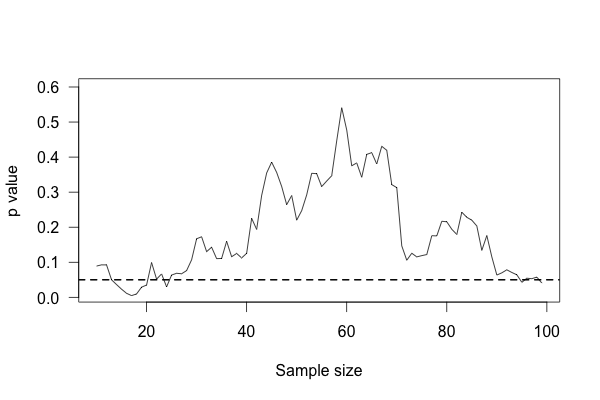
\includegraphics[width=0.8\textwidth]{sample-size}
    %\caption{}
    \label{fig9:sample-size}
\end{figure}
%%%%%%%%%%%%%%% end of figure %%%%%%%%%%%%%%%%%%%

Этот график показывает изменения \emph{p}-значения различий между группами в процессе сбора нами данных, а горизонтальная линия означает уровень значимости $p = 0,05$. На первый взгляд может показаться, что значимых различий нет. Тогда мы собираем больше данных и делаем противоположный вывод. Если бы мы решили остановиться, это было бы заблуждением: мы были бы убеждены в том, что между группами существует значимое различие, в то время как в реальности его нет. Если мы соберём еще больше данных, мы поймем, что были неправы - но в таком случае, есть шанс снова получить ложноположительный результат.  

Можно ожидать, что такое изменение \emph{p}-значения не должно происходить, поскольку реальных различий между группами нет. В конце концов, сбор большего количества данных не должно ухудшать наши выводы, разве нет? И действительно, если мы проведем эксперимент еще раз, мы можем обнаружить, что в начале у групп нет значимых различий, и они не появляются, пока мы собираем данные, или, что сначала у групп есть огромные различия, но в процессе эксперимента они быстро уменьшаются до нуля. Но если мы подождем достаточно долго и будем сравнивать различия после каждого измерения, в конечном итоге мы можем пересечь любую произвольную линию статистической значимости, даже если в реальности различий не будет. Обычно мы не в состоянии собирать данные на бесконечных выборках, поэтому в реальности такого не происходит, но неудачно  составленные и плохо применяемые правила остановки все равно значимо увеличивают количество ложноположительных результатов. \cite{simmons_false-positive_2011}  


Современные клинические испытания часто требуют регистрации используемых статистических протоколов заранее, и, как правило, выбирают только некоторые резальтаты измерения, которые потом тестируют, вместо того, чтобы тестировать после каждого измерения. Это вызывает лишь небольшое увеличение ложноположительных результатов, которое можно корректировать тщательно подобранными уровнями значимости и используя сложные статистические методы.\cite{todd_interim_2001} Но в сферах науки, где протоколы исследования не регистрируются и у исследователей есть возможность выбирать любые методы, которые они считают подходящими, всегда найдется место для таких ошибок.


\section{Преувеличение истины}
\label{chp7:truthinflation}

У медицинских экспериментов также существует тенденция иметь неадекватную статистическую мощность для определения умеренных различий между лекарствами. И они стремятся остановить исследование, как только обнаруживается какой-то результат, но у них не хватает мощности, чтобы обнаружить различия.

Предположим, что лекарство снижает проявление симптомов на 20\% по сравнению с плацебо, но эксперимент, в котором вы пытаетесь это проверить, не имеет адекватной статистической мощности, чтобы определить это различие. Мы знаем, что результаты небольших исследований могут варьировать: удачно собрать в одном эксперименте десять пациентов с более короткой продолжительностью простуды, чем в среднем, легко, но гораздо сложнее собрать десять тысяч таких людей.   

А теперь представьте, что вы проводите множество таких же экспериментов. Иногда вам попадаются не такие удачливые пациенты, и поэтому вы не замечаете никакого статистически значимого улучшения от действия вашего лекарства. Иногда пациенты имеют типично средние показатели, и можно рпонаблюдать снижение симптомов на 20\% благодаря лекарству, но вы игнорируете эти результаты, поскольку у вас недостаточно данных для того, чтобы считать такое улучшение статистически значимым. Иногда пациентам везёт, и их симптомы снижаются более, чем на 20\%, и тогда вы останавливаете эксперимент и говорите:``Смотрите! Лекарство работает!'' 

Вы правильно сделали вывод, что лекарство эффективно, но вы преувеличили размер эффекта. Вы ошибочно поверили в то, что лекарство более эффективно, чем оно есть на самом деле. 

Это часто встречается в фармакологических испытаниях, эпидемиологических исследованиях, исследованиях связей на генном уровне (``ген А является причиной условия В''), психологических исследованиях и в некоторых наиболее цитируемых статьях в медицинской литературе. \cite{ioannidis_why_2008,ioannidis_contradicted_2005} В сферах, где испытания могут проводиться быстро и большим количеством независимых исследователей (как, например, исследования генных связей), самые первые опубликованные результаты зачастую оказываются крайне противоречивыми, поскольку небольшие размеры экспериментов и потребность в статистической значимости приводят к тому, что лишь наиболее выдающиеся результаты в итоге публикуются. \cite{ioannidis_early_2005} 

В качестве бонуса, преувеличение истины можно объединять с правилами предварительной остановки. Если большинство лекарств в клинических испытаниях не настолько эффективны, чтобы оправдать предварительную остановку испытаний, в таком случае большинство экспериментов, остановленных предварительно, будут результатом участия удачливых пациентов, а не действия выдающихся лекарств, - и, останавливая эксперимент, мы фактически лишаем себя возможности собрать дополнительные данные, чтобы это опровергнуть. Обзоры научной литературы сравнивали исследования, остановленные предварительно,  

As a bonus, truth inflation can combine forces with early stopping rules. If most drugs in clinical trials are not quite so effective to warrant stopping the trial early, then many trials stopped early will be the result of lucky patients, not brilliant drugs – and by stopping the trial we have deprived ourself of the extra data needed to tell the difference. Reviews have compared trials stopped early with other studies addressing the same question which did not stop early; in most cases, the trials stopped early exaggerated the effects of their tested treatments by an average of 29%.3

Of course, we do not know The Truth about any drug being studied, so we cannot tell if a particular study stopped early due to luck or a particularly good drug. Many studies do not even publish the original intended sample size or the stopping rule which was used to justify terminating the study.43 A trial’s early stoppage is not automatic evidence that its results are biased, but it is a suggestive detail.

\section{Little extremes}
\label{chp7:littleextremes}

Suppose you’re in charge of public school reform. As part of your research into the best teaching methods, you look at the effect of school size on standardized test scores. Do smaller schools perform better than larger schools? Should you try to build many small schools or a few large schools?

To answer this question, you compile a list of the highest-performing schools you have. The average school has about 1,000 students, but the top-scoring five or ten schools are almost all smaller than that. It seems that small schools do the best, perhaps because of their personal atmosphere where teachers can get to know students and help them individually.

Then you take a look at the worst-performing schools, expecting them to be large urban schools with thousands of students and overworked teachers. Surprise! They’re all small schools too.

What’s going on? Well, take a look at a plot of test scores vs. school size:


\newpage % делаем разрыв, чтобы картинка была первой на след странице

%%%%%%%%%%%%%% figure 10 %%%%%%%%%%%%%%%%%%5
\begin{figure}[h!]
    \centering
    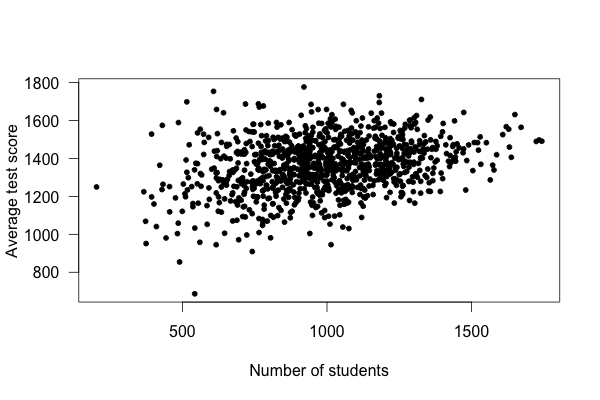
\includegraphics[width=0.5\textwidth]{school-size}
    %\caption{}
    \label{fig9:school-size}
\end{figure}
%%%%%%%%%%%%%%% end of figure %%%%%%%%%%%%%%%%%%%
%%%%%%%%%%%%%%%%%%%%%%%%%%%55
%http://www.statisticsdonewrong.com/_images/school-size.png
%%%%%%%%%%%%%%%%%%%%%%%%%%%%%%%%

Smaller schools have more widely varying average test scores, entirely because they have fewer students. With fewer students, there are fewer data points to establish the “true” performance of the teachers, and so the average scores vary widely. As schools get larger, test scores vary less, and in fact increase on average.

This example used simulated data, but it’s based on real (and surprising) observations of Pennsylvania public schools.59

Another example: In the United States, counties with the lowest rates of kidney cancer tend to be Midwestern, Southern and Western rural counties. How could this be? You can think of many explanations: rural people get more exercise, inhale less polluted air, and perhaps lead less stressful lives. Perhaps these factors lower their cancer rates.

On the other hand, counties with the highest rates of kidney cancer tend to be Midwestern, Southern and Western rural counties.

The problem, of course, is that rural counties have the smallest populations. A single kidney cancer patient in a county with ten residents gives that county the highest kidney cancer rate in the nation. Small counties hence have vastly more variable kidney cancer rates, simply because they have so few residents.21

